\documentclass{beamer}

\usepackage{rbstyle}
\title{Big Data}
\subtitle{Projekt: Amazonreviews}
\author[Nameshort]{Matthias Körschens \& Kevin Reinke}
\institute{Friedrich-Schiller-Universität Jena}

\begin{document}
	\nofooter{
		\frame{\titlepage}
	}
	\begin{frame}
		\tableofcontents
	\end{frame}
	\section{Zielsetzung}
	\begin{frame}
	\frametitle{Ziel}
	Explorative Datenanalyse von AmazonReviews. Im speziellen die Verteilung der Reviews, das Bewertungsverhalten der Nutzer sowie Clustern von Nutzern.
	\end{frame}
	\section{Datensatz}
	\begin{frame}
	\begin{itemize}
	\item AmazonReviews von \url{http://jmcauley.ucsd.edu/data/amazon/}
	\item Zeitraum: Mai 1996 bis Juni 2014
	\item Teildatensatz: Elektronik
	\item 4,7 GB
	\item 7,8 Millionen Reviews und etwa 4,2 Millionen Nutzern
	\item Format: JASON
	\end{itemize}
	\end{frame}
	\begin{frame}
	\frametitle{Beispiel}
	\{\\
  "reviewerID": "A2SUAM1J3GNN3B",\\ 
  "asin": "0000013714", \\
  "reviewerName": "J. McDonald", \\
  "helpful": [2, 3], \\
  "reviewText": "I bought this for my husband who plays the piano. He is having a wonderful time playing these old hymns. The music is at times hard to read because we think the book was published for singing from more than playing from. Great purchase though!", \\
  "overall": 5.0, \\
  "summary": "Heavenly Highway Hymns", \\
  "unixReviewTime": 1252800000, \\
  "reviewTime": "09 13, 2009" \\
  \}
	\end{frame}
	\section{Strukturen}
	\begin{frame}
	\frametitle{Wie sind die Reviews verteilt?}
	\begin{itemize}
	\item den Nutzern ihre eigenen Reviews zugeordnet
	\item Die meisten Nutzer bewerten wenig. 2,88 von 4,2 Millionen Nutzern die nur ein einziges Review abgaben.
	\item Zusammenhang exponentiell (Zipfsche Gesetzt)
	\end{itemize}
	\end{frame}
	
	\begin{frame}
	\begin{figure}[H]
\centering
    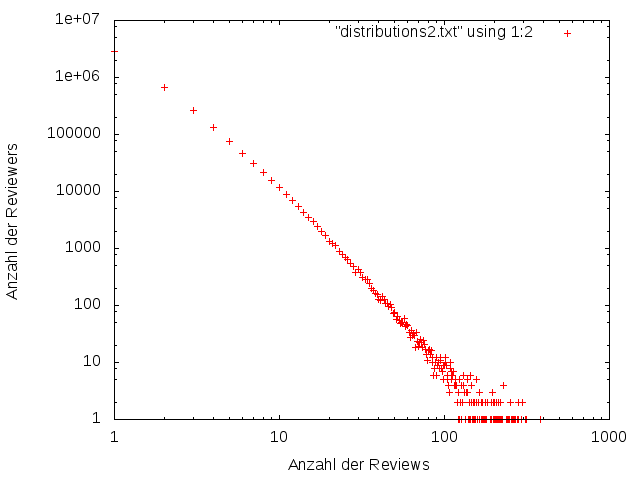
\includegraphics[width=0.8\textwidth]{bild.png}
    \caption{Reviewverteilung}
\end{figure}
	\end{frame}
	
	\begin{frame}
	\frametitle{Reviewerverhalten bei steigener Reviewanzahl}
	\begin{itemize}
	\item Gruppierung der Nutzer nach Reviewanzahl beibehalten
	\item Merkmale: Bewertung, Wortzahl, Zeichenzahl, Hilfreich
	\item innerhalb einer Gruppe Merkmale arithmetisch mitteln
	\end{itemize}
	\end{frame}
	
		\begin{frame}
	\begin{figure}[H]
\centering
    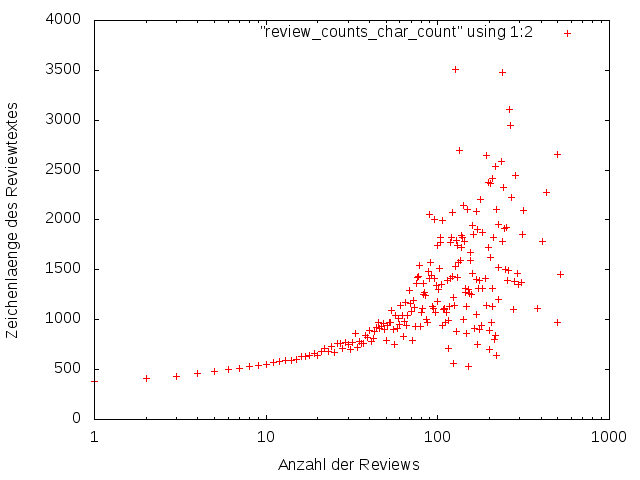
\includegraphics[width=0.8\textwidth]{_results/char_count2.png}
    \caption{Reviewverteilung}
\end{figure}
	\end{frame}
	
		\begin{frame}
	\begin{figure}[H]
\centering
    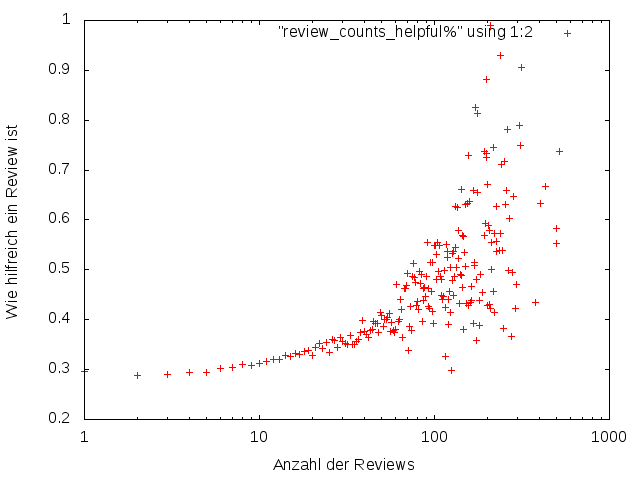
\includegraphics[width=0.8\textwidth]{_results/helpfull_count2.png}
    \caption{Reviewverteilung}
\end{figure}
	\end{frame}
	
		\begin{frame}
	\begin{figure}[H]
\centering
    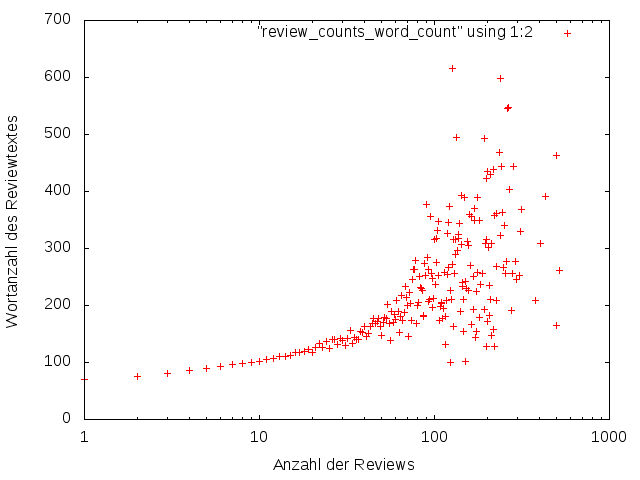
\includegraphics[width=0.8\textwidth]{_results/word_count2.png}
    \caption{Reviewverteilung}
\end{figure}
	\end{frame}
	
		\begin{frame}
	\begin{figure}[H]
\centering
    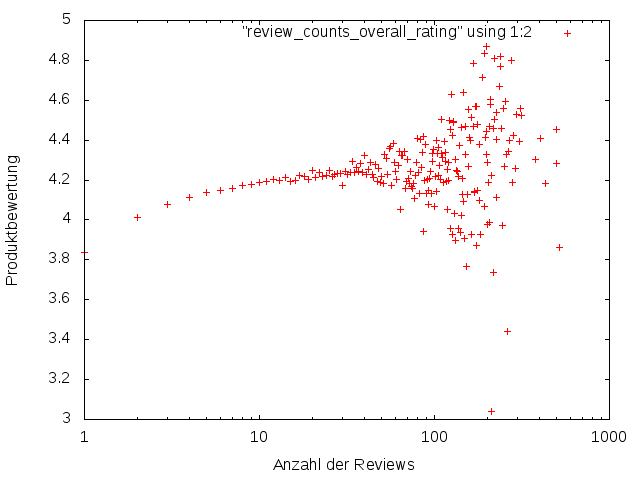
\includegraphics[width=0.8\textwidth]{_results/rating_count.png}
    \caption{Reviewverteilung}
\end{figure}
	\end{frame}
	
	\begin{frame}
	\frametitle{Textlänge und Produktbewertung}
	\begin{itemize}
	\item Analog über Textlänge Gruppiert
	\item Produktbewertungen je Gruppe gemittelt
	\item ein Bewertungstief bei ca 180 Wörtern
	\item ab 1000 Wörtern ungenau
	\end{itemize}
	\end{frame}
		
	\begin{frame}
		\begin{figure}[H]
    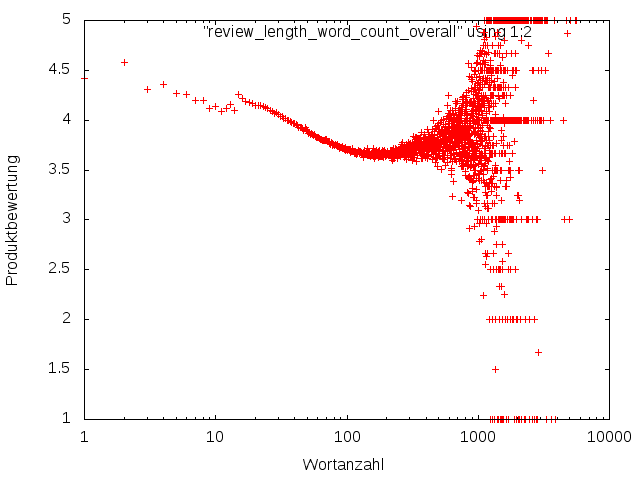
\includegraphics[width=0.8\textwidth]{_results/word_rating.png}
    \caption{Reviewverteilung}
	\end{figure}
	\end{frame}
	
	\begin{frame}
		\begin{figure}[H]
    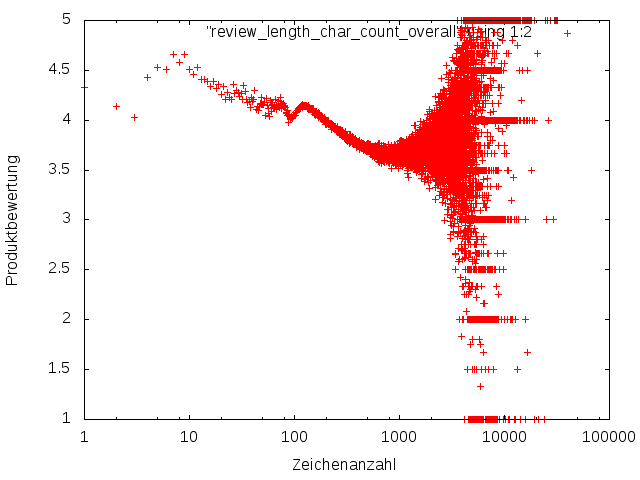
\includegraphics[width=0.8\textwidth]{_results/char_rating.png}
    \caption{Reviewverteilung}
	\end{figure}
	\end{frame}
	
	\section{Clustern}
	\begin{frame}
	\begin{itemize}
	\item Nutzer mit seinen Reviews erhält Merkmalsvektor
	\item Merkmale
	\begin{itemize}
	\item Wortanzahl des Bewertungstextes
	\item Zeichenanzahl des Bewertungstextes
	\item Zeitstempel des Reviews
	\item Zeichenanzahl des Reviewtitels
	\item wie hilfreich das Review war prozentual
	\item wieviele das Review ingesamt nützlich fanden
	\item Produktbewertung
	\end{itemize}
	\item Clusterverfahren, mit Distanzmaß zwischen allen Reviewern$\rightarrow$ verworfen
	\item PCA
	\item K-Means mit $k=2,44$ und $65$ gewählt
	\end{itemize}
	\end{frame}
	
	\begin{frame}
	\centering
	{\Huge Danke}
	\end{frame}
	
	
\end{document}